\subsection{Data Weighting}
\label{sec:DataWeight}


In 2015 there was a CAPAM workshop dedicated to data-weighting. Description of the workshop can be found on the \href{http://capamresearch.org/data-weighting/workshop}{CAPAM} website. The presentations from the workshop are available through that website and many of them were included in a special issue of \href{https://sciencedirect.com/journal/fisheries-research/vol/192}{Fisheries Research}.


Currently, there are three main methods for weighting length and data applied for U.S. West Coast assessments using Stock Synthesis.

\begin{enumerate}
	\item \textbf{McAllister - Ianelli}: Effective sample size is calculated from fit of observed to expected length or age compositions. Tuning algorithm is intended to make the arithmetic mean of the input sample size equal to the harmonic mean of the effective sample size \citep{mcallister_bayesian_1997}.
	
	\item \textbf{Francis}: Based on variability in the observed mean length or age by year, where the sample sizes are adjusted such that the fit of the expected mean length or age should fit within the uncertainty intervals at a rate which is consistent with variability expected based on the adjusted sample sizes (Method "TA1.8") \citep{francis_data_2011}
	
	\item \textbf{Dirichlet-Multinomial}: A new likelihood (as opposed to the standard multinomial) which includes an estimable parameter (theta) which scales the input sample size. In this case, the term "Effective sample size" has a different interpretation than in the McAllister-Ianelli approach \citep{thorson_model-based_2017}.
\end{enumerate}

\myparagraph{Applying the methods}

%\subsubsection{McAllister-Ianelli}
\myparagraph{McAllister-Ianelli}
The "Length\_Comp\_Fit\_Summary" and "Age\_Comp\_Fit\_Summary" sections in the Report file include information on the harmonic mean of the effective sample size and arithmetic mean of the input sample size used in this tuning method. In the r4ss package, these tables are returned by the \texttt{SS\_output} function as \texttt{ \$Length\_comp\_Eff\_N\_tuning\_check} and \texttt{ \$Age\_comp\_Eff\_N\_tuning\_check}.

A convenient way to process these values into the format required by the control file is to use the function:

\texttt{ SS\_tune\_comps(replist, option = "MI") }

where the input "replist" is the object created by \texttt{SS\_output}. This function will return a table and also write a matching file called "suggested\_tuning.ss" to the directory where the model was run.

For models using SS version 3.30, the table created by \texttt{SS\_tune\_comps} can be pasted into the bottom of the control file in the section labeled "Input variance adjustments", followed by the terminator line which indicates the end of the section. 

%Here's an example of the first few rows of the table followed by the terminator line (not added by the function):

%\begin{center}
%	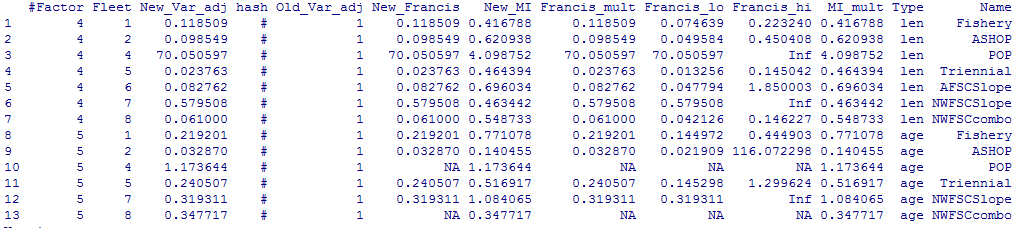
\includegraphics[scale = 0.6]{appendixB_sstune}\\
%\end{center}

Also see the help page for the r4ss function \texttt{SS\_varadjust} which can be used to automatically write a new control file if you want to streamline the process of applying multiple iterations of this tuning method.

If the tuning has been implemented, the green lines in the figure below would approximately intersect at a point which is on the black 1-to-1 diagonal line in this figure created by the r4ss function \texttt{SS\_plots}.

\begin{figure}[h]
	\begin{center}
		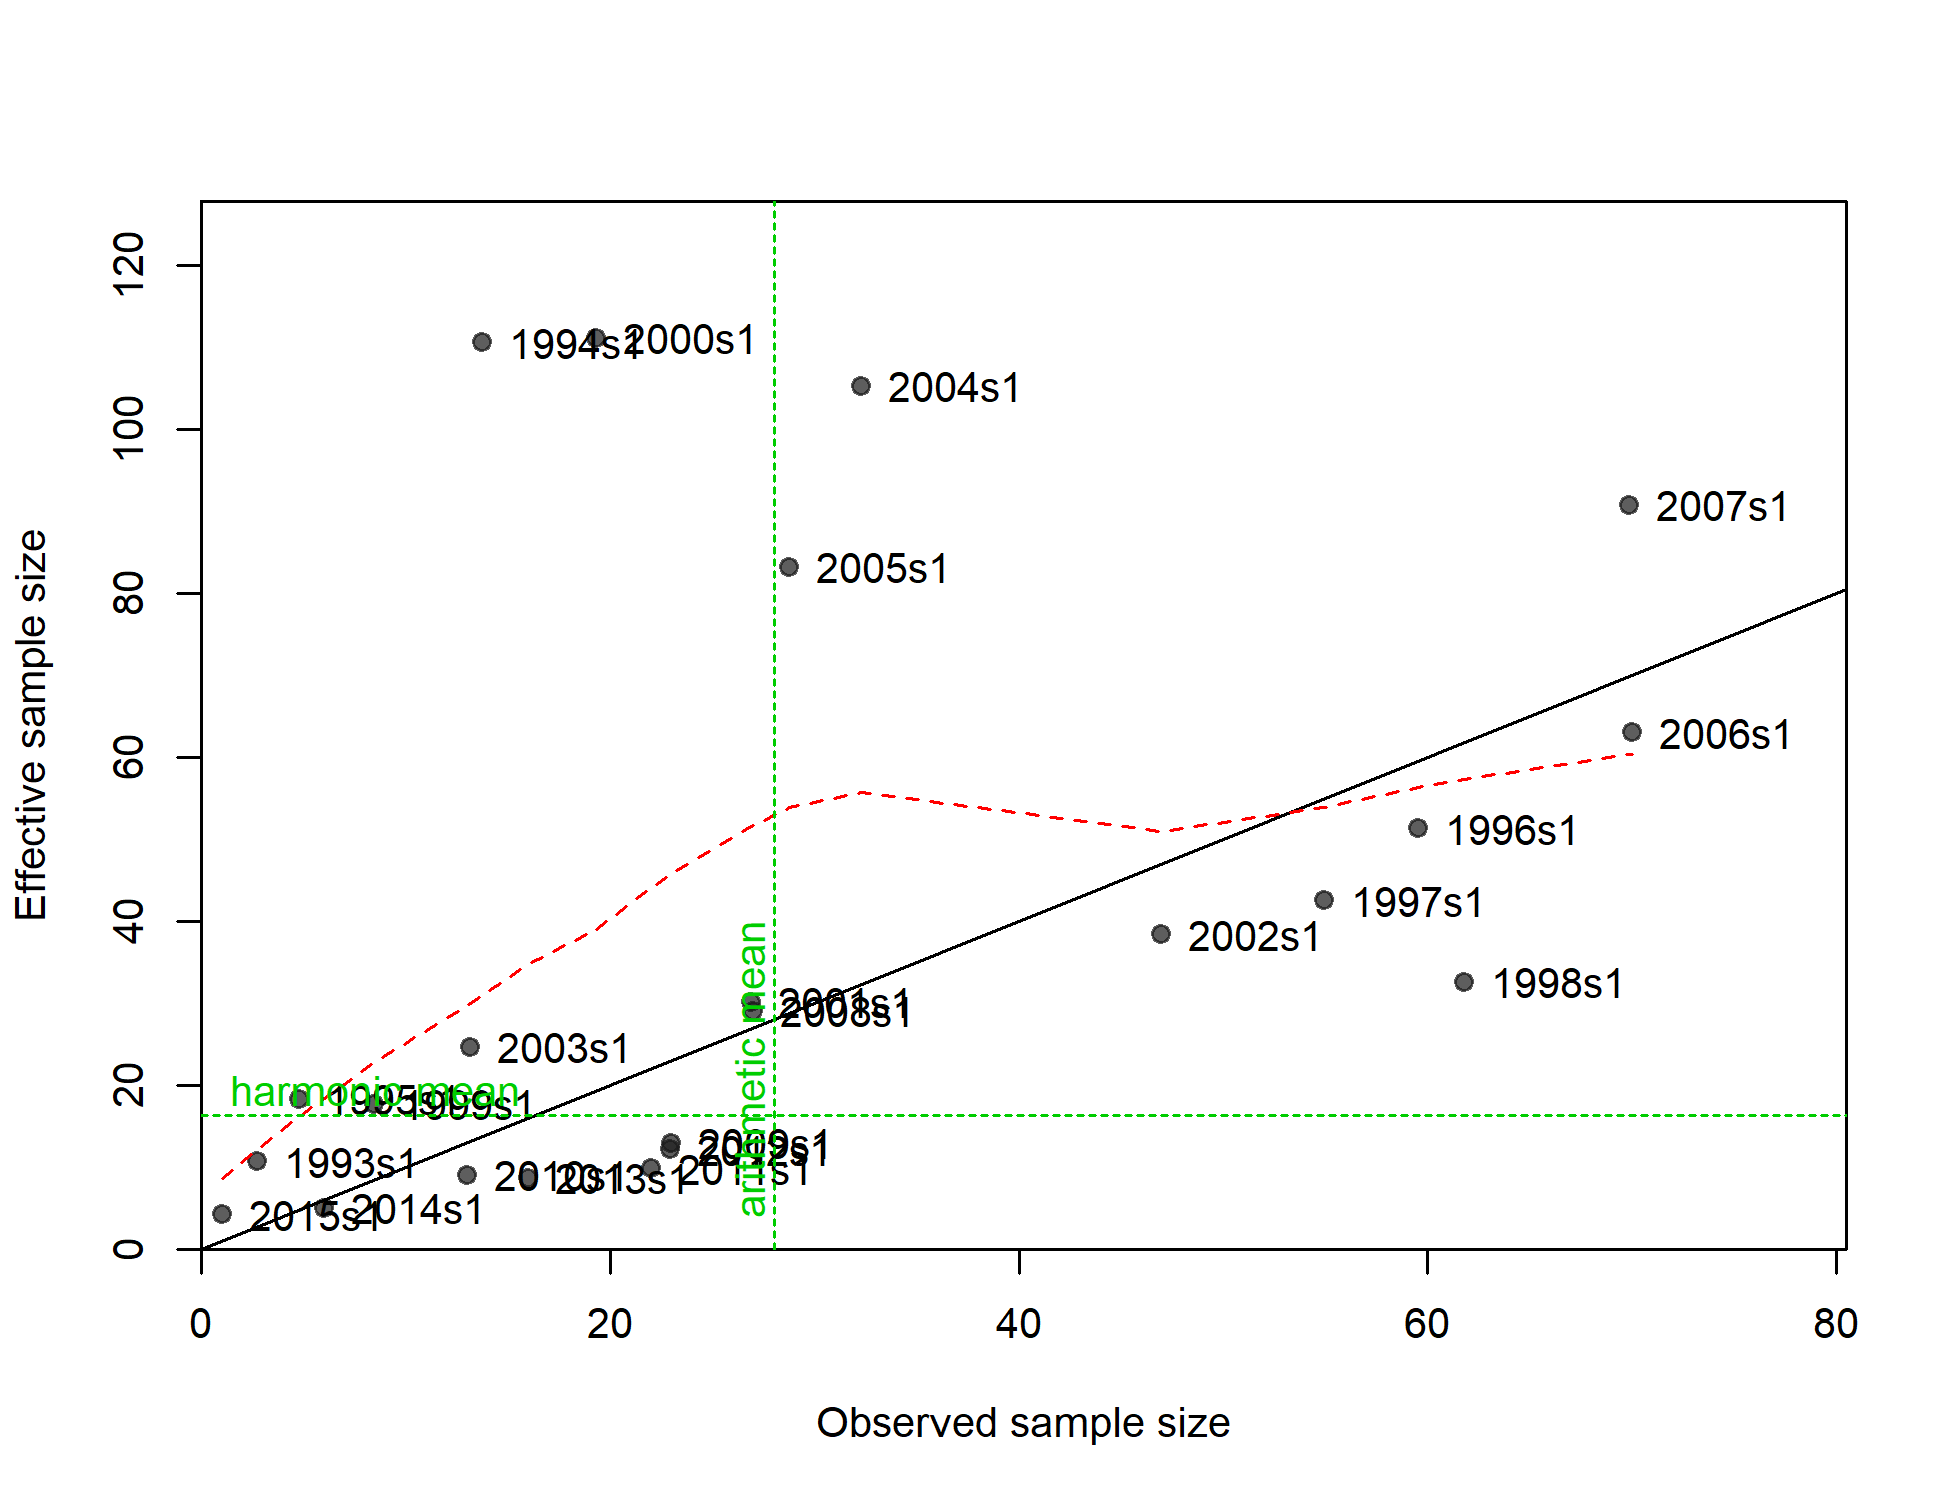
\includegraphics[scale = 0.65]{appendixB_McAllister_Ianelli}\\
	\end{center}

	\caption{ The relationship between the observed sample size (the input sample number) versus the effective sample size where the effective sample size is the product of the input sample size and the data weighting applied to the data set. }
	\label{(fig:mcallister)}
\end{figure}

There are a couple of challenges posed by the McAllister-Ianelli data-weighting approach:
\begin{enumerate}
	\item Subjective choice of how many iterations to take to achieve adequate convergence. Often just one iteration is applied.
	
	\item Takes time to implement so tuning is rarely repeated during retrospective or sensitivity analyses.
\end{enumerate}

%\subsubsection{Francis}
\myparagraph{Francis}

Implementation: recommended adjustments are calculated by the r4ss functions \texttt{SSMethod.TA1.8} and \texttt{SSMethod.Cond.TA1.8}. These functions are rarely used alone but are called by the \texttt{SS\_plots} function when making plots like the one below. For SS v.3.30 models, the simplest way to get the adjustments in the format required by the control file is to use the \texttt{SS\_tune\_comps} function (described above under the McAllister-Ianelli method), but with a different option specified: 

\texttt{SS\_tune\_comps(replist, option = "Francis")}

The figure below shows the estimated 95\% intervals around the observed mean length by year based on the input sample size (thick lines) and the increase in that uncertainty which would occur if the sample sizes were adjusted according to the proposed multiplier.

\begin{figure}[h]
	\begin{center}
		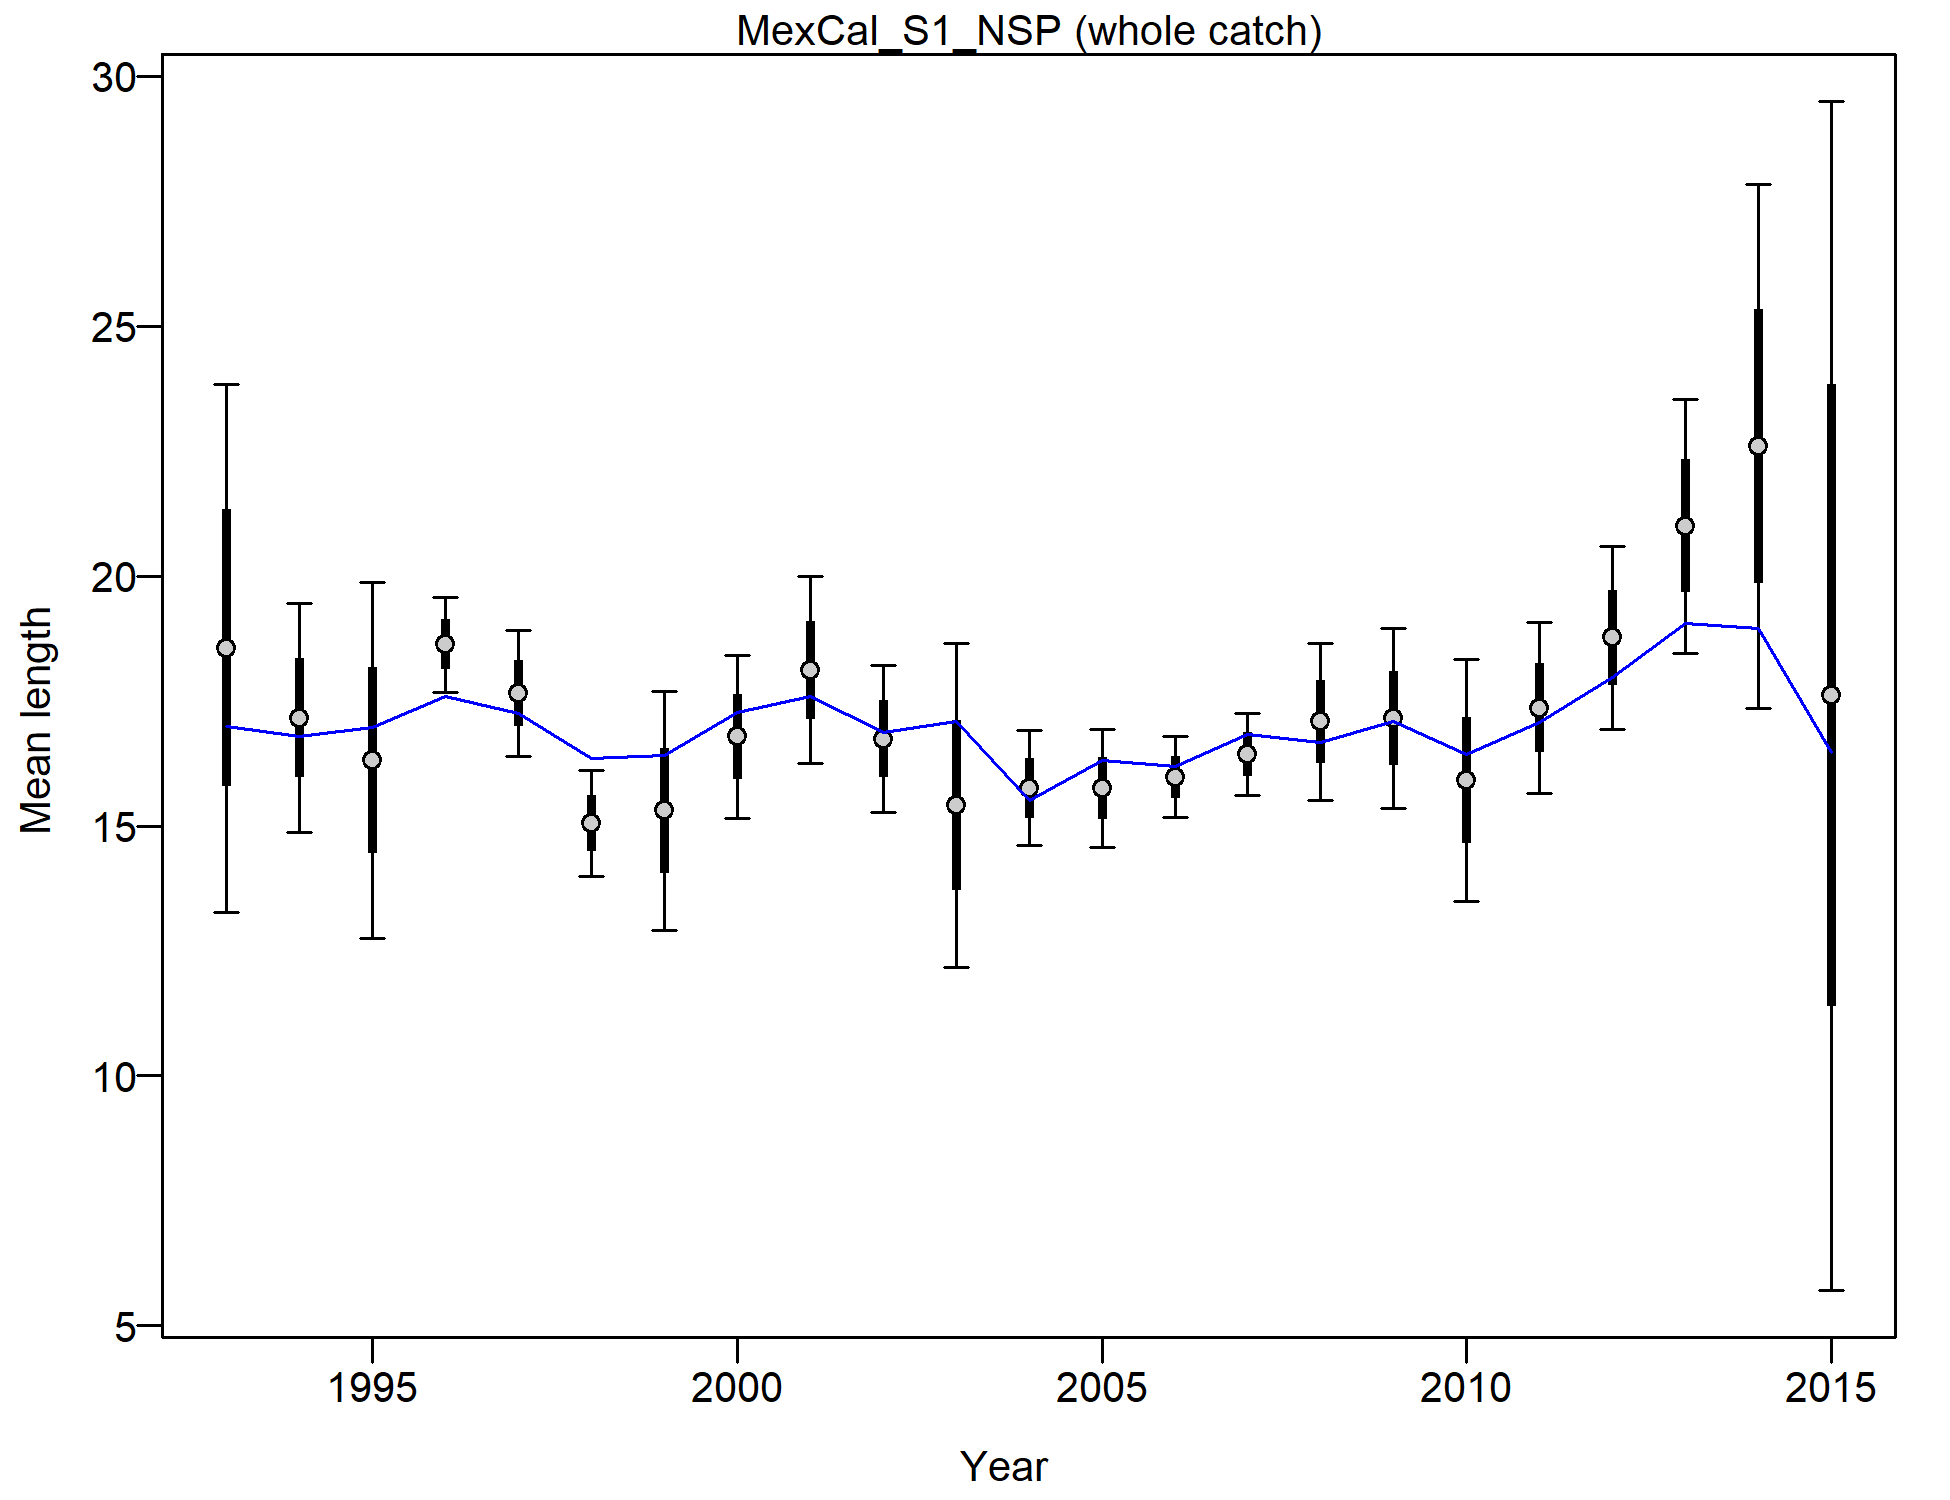
\includegraphics[scale = 0.15]{appendixB_Francis}\\
	\end{center}
	\caption{The mean length of the length samples for each year from Fleet 1 (called the MexCal S1 NSP fleet) with 95\% confidence intervals based on current samples sizes using the Francis data weighting method (referred to as TA1.8). Thinner intervals with capped ends show result of further adjusting sample sizes based on suggested multiplier, 0.2739, with 95\% interval (0.1661-0.6305) for length data from Fleet 1. The blue line shows the expected variation of the mean length across years.}
	\label{fig:francis}
	%\figurename{name}
\end{figure}



There are a several of challenges posed by the Francis data-weighting approach:
\begin{enumerate}
	\item Subjective choice of how many iterations to take to achieve adequate convergence. Often just one iteration is applied.
	
	\item Takes time to implement so tuning is rarely repeated during retrospective or sensitivity analyses.
	
	\item Recommended adjustment can be sensitive to outliers (remove a few years of anomalous composition data can lead to large change in recommended adjustment).
\end{enumerate}

%\subsubsection{Dirichlet-Multinomial}
\myparagraph{Dirichlet-Multinomial}

Change the choice of likelihood and set parameter choices in the data file:

\begin{itemize}
	\item In the specification of the length and/or age data, change "CompError" column in age and length comp specifications from 0 to 1 and "ParmSelect" from 0 to a sequence of numbers from 1 to N where N is the total number of combinations of fleet and age/length.
	
	\item Resulting input should look similar to:
	\begin{center}
		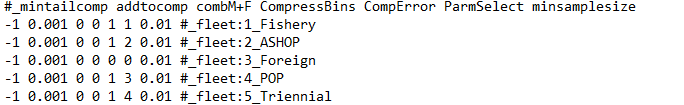
\includegraphics[scale = 0.75]{appendixB_DM_setup}\\
	\end{center}
	
	\item The ParmSelect column can also have repeated values so that multiple fleets share the same log(theta) parameter.
	
	\item If you have both length and age data, the ParmSelect should have separate numbers for each, e.g. 1 and 2 for the length comps and 3 and 4 for the age comps for the same two fleets.
	
\end{itemize}

Add parameter lines to the control file:

\begin{itemize}
	\item Add as many parameter lines as the maximum numbers in the ParmSelect column. The new parameter lines go after the main selectivity parameters but before any time-varying selectivity parameters
	
	\item Jim Thorson initially recommended bounds of -5 to 20, with a starting value of 0
	(which corresponds to a weight of about 50\% of the input sample size). However, parameter estimates above 5 are associated with 99-100\% weight with little information in the likelihood about the parameter value. Therefore, an upper bound of 5 may help identify cases that otherwise would have convergence issues.
	
	\item Example parameter lines are below: 
		\begin{center}
			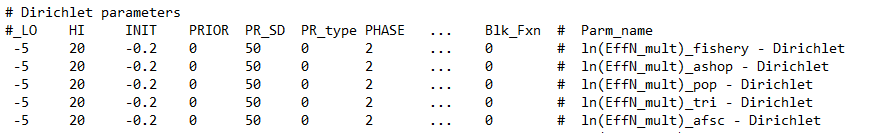
\includegraphics[scale = 0.70]{appendixB_DM_parameters}\\
		\end{center}
	
	\item Reset any existing variance adjustments factors that might have been used for the McAllister-Ianelli or Francis tuning methods. In 3.24 this means setting the values to 1, in SS version 3.30, you can simply delete or comment-out the rows with the adjustments.
\end{itemize}

The \texttt{SS\_output} function in r4ss returns table like the following:

\begin{center}
	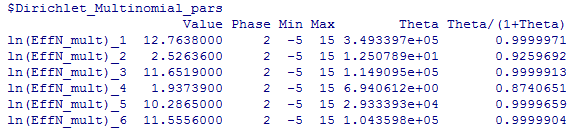
\includegraphics[scale = 1]{appendixB_DM_output}\\
\end{center}

The ratio shown in the final column is the estimated multiplier which can be compared to the sample size adjustment estimated in the other tuning methods above (the New\_Var\_adj column in the table produced by the \texttt{SS\_tune\_comps} function in r4ss).

If the reported $\theta/(1+\theta)$ ratio is close to 1.0, that indicates that the model is trying to tune the sample size as high as possible. In this case, the $ln(\theta)$ parameters should be fixed at a high value, like the upper bound of 20, which will result in 100\% weight being applied to the input sample sizes. An alternative would be to manually change the input sample sizes to a higher value so that the estimated weighting will be less than 100%.

%There is also information about this result produced in the plots created by the \texttt{SS\_plots} function:

%\begin{center}
%	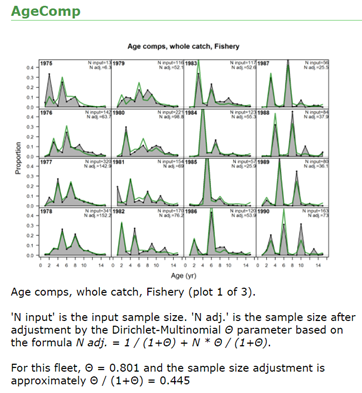
\includegraphics[scale = 1]{appendixB_DM}\\
%\end{center}

There are a several of challenges posed by the Dirichlet-Multinomial data-weighting approach:
\begin{enumerate}
	\item Not yet widely used so little guidance is available.
	
	\item Does not allow weights above 100\% (by design) so it is not yet clear how best to deal with the situation when the estimated weight is close to 100\%.
	
	\item Parameterization has potential to cause convergence issues or inefficient MCMC sampling when weights are close to 100\% (Jim Thorson has proposed a prior distribution that may help with this, but has not yet been tested).
\end{enumerate}